\documentclass[11pt]{article}

\usepackage[margin=1in]{geometry}
\usepackage{amsmath,amssymb,amsthm,mathtools}
\usepackage{booktabs}
\usepackage{enumitem}
\usepackage{tikz}
\usetikzlibrary{arrows.meta,positioning,calc}
\usepackage{microtype}
\usepackage{natbib}
\usepackage{xcolor}
\usepackage[colorlinks=true,allcolors=blue!45!black]{hyperref}

\newtheorem{theorem}{Theorem}
\newtheorem{proposition}{Proposition}
\newtheorem{lemma}{Lemma}
\newtheorem{corollary}{Corollary}
\theoremstyle{definition}
\newtheorem{definition}{Definition}
\theoremstyle{remark}
\newtheorem{remark}{Remark}

\newcommand{\E}{\mathbb E}
\newcommand{\calE}{\mathcal E}
\newcommand{\calI}{\mathcal I}
\newcommand{\ind}{\mathbf 1}

\title{\bfseries Announced Escalation with Strategic Drivers\\
\large A Two-Period Model with Latent Market Thickness}
\author{}
\date{}

\begin{document}
\maketitle

\begin{abstract}
We study a platform that commits to a first-period payment and a higher
failure-contingent rescue payment.  The platform observes market thickness but
not realized supply.  Riders decide whether to post and, after an initial
failure, whether to abandon, repeat the initial payment, or activate the rescue
payment.  Drivers privately observe their costs and may reject the initial
payment in anticipation of the rescue option.  We first characterize the
agents' anonymous symmetric pure-cutoff weak perfect Bayesian equilibrium
correspondence under an arbitrary announced escalation policy.  Each such
equilibrium is summarized by a scalar driver cutoff:
accepting immediately trades off current competition for assignment against
the possibility of being paid more after all rival drivers also wait.  We then
embed this equilibrium response in the platform's completion-maximization
problem.  A flat payment admits a unique symmetric cutoff equilibrium.  Starting
from any active flat payment, a small announced escalation strictly increases
completion whenever a positive mass of riders activates the rescue option.  In
the no-entry benchmark with positive incumbent survival, this local improvement
holds at every positive market thickness; when \(\beta>1/2\), it strictly
improves on the optimized flat payment.  The value of escalation nevertheless
vanishes in both very thin and very thick markets.
\end{abstract}

\section{Introduction}

Many platforms respond to an unfilled request by offering a higher payment in a
later round.  Announcing this escalation in advance improves the platform's
ability to rescue a request, but it also changes first-round behavior: a driver
may reject an acceptable payment today in the hope of receiving more after the
request fails.  The platform therefore cannot evaluate the second-round
payment while holding first-round acceptance fixed.

We study this tradeoff in a two-period model.  The platform observes a public
measure of market thickness, denoted by \(m\), but neither the platform policy
nor the agents' strategies can condition on the realized number of available
drivers.  The platform commits to an announced escalation policy
\((p_1,p_2)\), with \(p_2\ge p_1\).  A rider with private value decides whether
to post the request.  Drivers with private costs simultaneously decide whether
to accept the first payment.  If no driver accepts, the rider may abandon,
repeat \(p_1\), or activate \(p_2\).  Surviving incumbents and newly arriving
drivers then make terminal acceptance decisions.

Our organization follows the policy--equilibrium--optimization logic used in
the announced-pricing literature.  In particular, \citet{AvivPazgal2008}
first fix the seller's announced policy, solve the strategic customers'
threshold response, and only then evaluate and optimize the seller's policy.
We adopt the same order of analysis, while reversing the economic direction of
the policy.  Their consumers wait for a markdown and face a risk of stockout;
our drivers wait for an escalation and face the risk that another driver
accepts first.  The common methodological point is that an announced future
term must be evaluated through the equilibrium behavior it induces today.

The analysis proceeds in four steps.  First, fixing an announced escalation
policy, we solve the rider's continuation problem and the drivers' Bayesian
acceptance game.  The latter reduces to a scalar cutoff condition.  Second, we
insert that equilibrium response into the platform's completion probability
and define the platform's policy problem.  Third, we develop a flat-payment
benchmark and compare it with a small announced escalation.  Finally, we study
how the value of the policy changes with market thickness and with fresh supply
in the second period.

The main economic mechanism is a latent-competition wedge.  A driver who
accepts immediately competes with other accepting drivers for assignment.  Her
expected assignment share is
\[
  \phi(mp)=\frac{1-e^{-mp}}{mp}.
\]
A driver who waits reaches the rescue round only if every rival also rejects,
an event with probability \(e^{-mp}\).  Hence
\[
  \phi(mp)-e^{-mp}>0
  \qquad (m>0,\ p>0).
\]
When incumbents survive and a positive mass of riders activates rescue, this
strict difference makes a marginal rescue payment valuable even when no new
driver arrives in the second period.

\section{Model}
\label{sec:model}

\subsection{Operational setting and policy classes}

There is one potential request and two decision periods.  The public state is
market thickness \(m>0\).  Before any private information is observed, the
platform commits to an announced failure-contingent rescue policy in
\[
  \mathcal P^D
  =\{(p_1,p_2):0\le p_1\le p_2\le1\}.
\]
The payment \(p_j\) is paid by the rider to the selected driver.  We treat this
payment as a transfer and let the platform maximize the probability that a
potential request is completed.  A driver incurs cost only if she is selected;
an accepting driver who is not selected receives zero and incurs no cost.

The policy is \emph{announced}: after a first-period failure the platform
cannot revise \(p_2\).  The second payment is also \emph{optional}: the rider,
rather than the platform, decides whether to activate it.  A flat policy is the
nested class
\[
  \mathcal P^F=\{(p,p):0\le p\le1\}\subset\mathcal P^D.
\]
Thus the comparison is between two commitment protocols, not between an ex
ante commitment and an ex post price revision.

\subsection{Agents, latent supply, and information}

From the rider's perspective, the number of incumbent drivers is
\[
  N^I\sim\operatorname{Pois}(m).
\]
The realization of \(N^I\) is latent: it is not observed by the rider or by an
individual driver, and the announced policy cannot depend on it.

We use the standard Poisson-population convention.  Conditional on a focal
driver being present, the number of \emph{other} incumbent drivers remains
\(\operatorname{Pois}(m)\).  This assumption is the finite-market implication
of the Palm property of a Poisson population; it is not the ordinary
conditional distribution \(N^I-1\mid N^I\ge1\).

The rider's value is \(v\sim U[0,1]\).  A completion in period 1 gives value
\(v\), whereas a completion in period 2 gives value \(\beta v\), where
\(\beta\in(0,1)\).  Each driver has an independently drawn cost
\(c\sim U[0,1]\).  An incumbent remains available in period 2 with probability
\(\alpha\in[0,1]\).  In addition, a fresh pool
\[
  N^E\sim\operatorname{Pois}(\gamma m),\qquad \gamma\ge0,
\]
arrives in period 2, independently of all earlier uncertainty.

\subsection{Sequence of events}

The sequence is as follows.

\begin{enumerate}[label=\arabic*.]
  \item The platform observes \(m\) and announces \((p_1,p_2)\).
  \item The rider observes \(v\) and decides whether to post.
  \item The incumbent pool is realized.  Each incumbent observes her own cost
        and simultaneously accepts or rejects \(p_1\).
  \item If at least one driver accepts, the platform selects one accepting
        driver uniformly and the request is completed.
  \item If no driver accepts, the rider observes only the failure and chooses
        among abandoning, repeating \(p_1\), and activating \(p_2\).
  \item Incumbent survival and fresh entry are realized.  In the terminal
        period, all available drivers decide whether to accept the active
        payment.  If at least one accepts, one is selected uniformly.
\end{enumerate}

The rider does not observe the initial number of drivers, the number of active
rejections, the survival realization, or the number of fresh arrivals.

Figure~\ref{fig:extensive-form} gives the reduced extensive form.  It suppresses
the continuum of rider and driver types but preserves the order of moves, the
public failure signal, and the information that remains latent at each stage.

\begin{figure}[htbp]
\centering
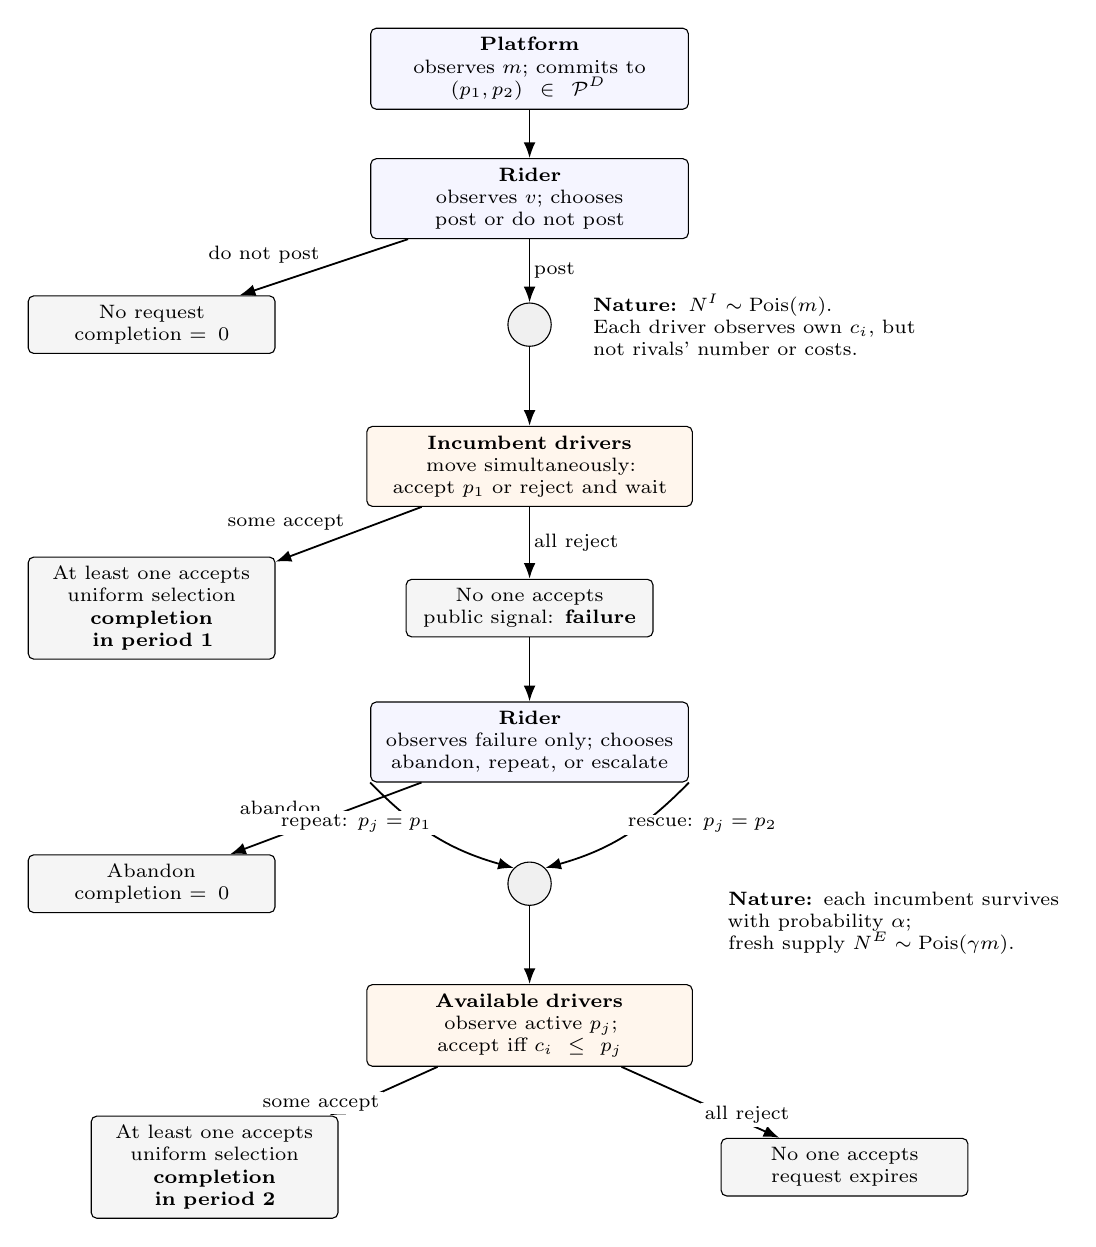
\begin{tikzpicture}[
  x=1cm,
  y=1cm,
  >={Latex[length=2mm]},
  flow/.style={->,line width=.65pt},
  decision/.style={draw,rounded corners=2pt,align=center,
    fill=blue!4,minimum height=8mm,text width=38mm,font=\scriptsize},
  driver/.style={draw,rounded corners=2pt,align=center,
    fill=orange!7,minimum height=9mm,text width=39mm,font=\scriptsize},
  terminal/.style={draw,rounded corners=2pt,align=center,
    fill=gray!8,minimum height=7mm,text width=29mm,font=\scriptsize},
  chance/.style={circle,draw,fill=gray!12,minimum size=5.5mm,inner sep=0pt},
  labeltext/.style={align=left,font=\scriptsize,text width=42mm},
  action/.style={font=\scriptsize,fill=white,inner sep=1.2pt}
]

\node[decision] (platform) at (0,0)
  {\textbf{Platform}\\observes $m$; commits to\\$(p_1,p_2)\in\mathcal P^D$};
\node[decision] (rider0) at (0,-1.65)
  {\textbf{Rider}\\observes $v$; chooses\\post or do not post};
\node[terminal] (nopost) at (-4.8,-3.25)
  {No request\\completion $=0$};

\node[chance] (nature1) at (0,-3.25) {};
\node[labeltext,right=4mm of nature1] (nature1text)
  {\textbf{Nature:} $N^I\sim\operatorname{Pois}(m)$.\\
   Each driver observes own $c_i$, but not rivals' number or costs.};

\node[driver] (drivers1) at (0,-5.05)
  {\textbf{Incumbent drivers}\\move simultaneously:\\accept $p_1$ or reject and wait};
\node[terminal] (complete1) at (-4.8,-6.85)
  {At least one accepts\\uniform selection\\\textbf{completion in period 1}};
\node[terminal] (failure) at (0,-6.85)
  {No one accepts\\public signal: \textbf{failure}};

\node[decision] (rider1) at (0,-8.55)
  {\textbf{Rider}\\observes failure only; chooses\\abandon, repeat, or escalate};
\node[terminal] (abandon) at (-4.8,-10.35)
  {Abandon\\completion $=0$};

\node[chance] (nature2) at (0,-10.35) {};
\node[labeltext,anchor=west] (nature2text) at (2.4,-10.85)
  {\textbf{Nature:} each incumbent survives with probability $\alpha$;\\
   fresh supply $N^E\sim\operatorname{Pois}(\gamma m)$.};
\node[driver] (drivers2) at (0,-12.15)
  {\textbf{Available drivers}\\observe active $p_j$;\\accept iff $c_i\le p_j$};
\node[terminal] (complete2) at (-4.0,-13.95)
  {At least one accepts\\uniform selection\\\textbf{completion in period 2}};
\node[terminal] (expire) at (4.0,-13.95)
  {No one accepts\\request expires};

\draw[flow] (platform) -- (rider0);
\draw[flow] (rider0) -- node[action,above left]{do not post} (nopost);
\draw[flow] (rider0) -- node[action,right]{post} (nature1);
\draw[flow] (nature1) -- (drivers1);
\draw[flow] (drivers1) -- node[action,above left]{some accept} (complete1);
\draw[flow] (drivers1) -- node[action,right]{all reject} (failure);
\draw[flow] (failure) -- (rider1);
\draw[flow] (rider1) -- node[action,above left]{abandon} (abandon);
\draw[flow] (rider1.south west) to[bend right=15]
  node[action,above left]{repeat: $p_j=p_1$} (nature2.north west);
\draw[flow] (rider1.south east) to[bend left=15]
  node[action,above right]{rescue: $p_j=p_2$} (nature2.north east);
\draw[flow] (nature2) -- (drivers2);
\draw[flow] (drivers2) -- node[action,below left]{some accept} (complete2);
\draw[flow] (drivers2) -- node[action,below right]{all reject} (expire);

\end{tikzpicture}
\caption{Reduced extensive form of the announced rescue game.  Decision boxes
identify the acting side; circles are chance moves.  Continuous type branches
and individual simultaneous driver actions are summarized inside their decision
nodes.  The public history consists of $m$, the announced policy, and whether
period 1 failed; realized driver counts, rivals' costs, survival, and fresh entry
remain latent.}
\label{fig:extensive-form}
\end{figure}

\subsection{Equilibrium and tie-breaking}

We study weak perfect Bayesian equilibria (WPBE) in anonymous, symmetric, pure
driver strategies.  Strategies are sequentially rational, and beliefs after a
first-period failure follow Bayes' rule.  Because a failure has positive
probability for every finite \(m\), the relevant posterior is reached on path.

The following tie-breaking rules make the equilibrium assessment single
valued at payoff ties.  A rider with \(v\ge p_1\) posts when indifferent,
whereas a rider with \(v<p_1\) does not post when indifferent.  At the failure
node, if all continuation actions yield zero, the rider repeats \(p_1\) when
\(\beta v-p_1\ge0\) and abandons otherwise.  When \(p_2=p_1\), repeat is
selected over the nominal escalation action.  We specify the action of a
cutoff driver directly when stating the equilibrium conditions.  The
repeat--abandon convention is substantive: when \(\gamma=0\) and \(a=p_1\),
rider types with \(v\ge p_1/\beta\) obtain zero from both actions, and their
choice to repeat affects a deviating driver's continuation payoff.

\section{Equilibrium Under an Announced Escalation Policy}
\label{sec:equilibrium}

We now fix \(m\) and an announced policy \((p_1,p_2)\).  Following the
leader--follower order of the game, we first solve the agents' continuation
behavior and then characterize first-period acceptance.

\subsection{Supply following a first-period failure}

Define
\[
  \phi(x)=
  \begin{cases}
    (1-e^{-x})/x, & x>0,\\
    1, & x=0.
  \end{cases}
\]
Suppose incumbents use a first-period cutoff \(a\in[0,p_1]\): a driver with
cost below \(a\) accepts, and a driver with cost above \(a\) rejects.

\begin{lemma}[Poisson competition]
\label{lem:poisson}
Under cutoff \(a\), the first-period completion probability conditional on
posting is \(1-e^{-ma}\).  A focal driver who accepts in period 1 receives the
assignment with expected share
\[
  \sigma_m(a)=\phi(ma).
\]
After a first-period failure, the number of drivers willing to accept payment
\(p_j\) in period 2 is Poisson with mean
\[
  \lambda_j(m,a)
  =m\bigl[\alpha(p_j-a)+\gamma p_j\bigr].
\]
Consequently, the period-2 coverage probability and a waiting incumbent's
expected assignment share are
\[
  C_j(m,a)=1-e^{-\lambda_j(m,a)},
  \qquad
  \widetilde s_{j,m}(a)=\phi(\lambda_j(m,a)).
\]
\end{lemma}

The result follows from Poisson splitting and thinning.  A failure reveals
that no incumbent with cost below \(a\) is present.  It does not change the
distribution of incumbents with costs in \((a,p_j]\).  Survival thins that
group by \(\alpha\), while fresh supply contributes an independent Poisson
group of mean \(\gamma m p_j\).

\subsection{The rider's equilibrium response}

Given \(a\), the expected payoff from posting is
\[
\begin{aligned}
\Pi(v;a)
={}&(1-e^{-ma})(v-p_1)\\
&+e^{-ma}
\max\bigl\{
0,\ C_1(m,a)(\beta v-p_1),\
C_2(m,a)(\beta v-p_2)
\bigr\}.
\end{aligned}
\]
Under our tie-breaking convention, the rider posts if and only if
\[
  v\ge p_1.
\]
Thus the posting mass is \(1-p_1\).

When \(C_2>C_1\), define the rider type indifferent between repeat and
escalation by
\[
  v_m^M(a)
  =
  \frac{C_2(m,a)p_2-C_1(m,a)p_1}
       {\beta[C_2(m,a)-C_1(m,a)]}.
\]
When \(C_2=C_1\), set \(v_m^M(a)=+\infty\).  Since
\[
  v_m^M(a)\ge\frac{p_2}{\beta}\ge\frac{p_1}{\beta},
\]
the continuation strategy takes a simple threshold form:
\[
\begin{cases}
\text{abandon}, & v<p_1/\beta,\\
\text{repeat }p_1, & p_1/\beta\le v<v_m^M(a),\\
\text{activate }p_2, & v\ge v_m^M(a).
\end{cases}
\]

Conditional on posting, let
\[
  \eta_m^R(a)
  =
  \frac{[\min\{v_m^M(a),1\}-p_1/\beta]^+}{1-p_1}
\]
and
\[
  \eta_m(a)
  =
  \frac{[1-v_m^M(a)]^+}{1-p_1}
\]
denote the masses that repeat and escalate.  Their sum is
\[
  \eta_m^R(a)+\eta_m(a)
  =
  \rho(p_1)
  :=
  \frac{[1-p_1/\beta]^+}{1-p_1}.
\]
The total continuation mass depends only on the first-period payment and
rider patience.  The cutoff, thickness, and rescue payment determine how this
mass is divided between repeat and escalation.

\subsection{The drivers' first-period game}

A driver with \(c\le p_1\) who accepts immediately obtains
\[
  U_m^A(c;a)=\phi(ma)(p_1-c).
\]
If she rejects, the request reaches period 2 only when all other first-period
drivers also reject.  Her waiting payoff is
\[
\begin{aligned}
U_m^W(c;a)
=e^{-ma}\alpha\Big[
&\eta_m^R(a)\phi(\lambda_1(m,a))[p_1-c]^+\\
&+\eta_m(a)\phi(\lambda_2(m,a))[p_2-c]^+
\Big].
\end{aligned}
\]
For \(c\le p_1\), define the accept-minus-wait difference
\[
\begin{aligned}
\Psi_m(c;a)
={}&\phi(ma)(p_1-c)\\
&-e^{-ma}\alpha\Big[
\eta_m^R(a)\phi(\lambda_1(m,a))(p_1-c)\\
&\hspace{31mm}
+\eta_m(a)\phi(\lambda_2(m,a))(p_2-c)
\Big].
\end{aligned}
\]
The relevant single-crossing property is immediate:
\[
  \frac{\partial\Psi_m(c;a)}{\partial c}
  \le
  -\phi(ma)+e^{-ma}\alpha\rho(p_1)<0
\]
whenever \(p_1>0\).  Hence lower-cost drivers have a strictly stronger
incentive to accept immediately.  Drivers with \(c>p_1\) reject because
accepting gives a negative payoff while waiting gives a nonnegative payoff.

Let
\[
  f_m(a;p_1,p_2):=\Psi_m(a;a).
\]

\begin{proposition}[Symmetric cutoff WPBE]
\label{prop:wpbe}
For every \(m>0\) and \(0\le p_1\le p_2\le1\), with \(p_1<1\), the announced
policy admits an anonymous symmetric pure-strategy cutoff WPBE.  The equilibrium
cutoff belongs to
\[
\calE_m^{\alpha,\gamma}(p_1,p_2)
=
\left\{
a\in[0,p_1]:
\begin{array}{ll}
f_m(0;p_1,p_2)\le0, & a=0,\\
f_m(a;p_1,p_2)=0, & 0<a<p_1,\\
f_m(p_1;p_1,p_2)\ge0, & a=p_1
\end{array}
\right\}.
\]
This correspondence is nonempty and compact.
\end{proposition}

At \(a=0\), all types reject.  At an interior cutoff, types below \(a\)
accept and types above \(a\) reject.  At \(a=p_1\), all types with
\(c\le p_1\) accept.  Existence follows from continuity and
\[
  f_m(p_1;p_1,p_2)
  =
  -e^{-mp_1}\alpha\eta_m(p_1)
   \phi(\lambda_2(m,p_1))(p_2-p_1)
  \le0.
\]
If \(f_m(0)\le0\), reject-all is an equilibrium.  If \(f_m(0)>0\) and
\(f_m(p_1)<0\), continuity gives an interior root; if \(f_m(p_1)=0\), the
boundary cutoff \(a=p_1\) is an equilibrium.

\section{The Platform's Policy Problem}
\label{sec:platform}

Having solved the follower game for a fixed policy, we now evaluate the
platform's objective.  Given a cutoff equilibrium \(a\), the unconditional
completion probability is
\[
\begin{aligned}
M_m^{\alpha,\gamma}(p_1,p_2;a)
=(1-p_1)\Big[
&1-e^{-ma}\\
&+e^{-ma}\{
\eta_m^R(a)C_1(m,a)+\eta_m(a)C_2(m,a)
\}
\Big].
\end{aligned}
\]
The expression separates the posting margin from execution:
\[
\underbrace{1-p_1}_{\text{posting}}
\times
\left[
\underbrace{1-e^{-ma}}_{\text{first-period completion}}
+
\underbrace{e^{-ma}(\eta_m^R C_1+\eta_m C_2)}
_{\text{failure-contingent rescue}}
\right].
\]

An arbitrary policy may admit more than one symmetric cutoff equilibrium.
Accordingly, define its implementable completion set by
\[
  \calI_m(p_1,p_2)
  =
  \left\{
  M_m^{\alpha,\gamma}(p_1,p_2;a):
  a\in\calE_m^{\alpha,\gamma}(p_1,p_2)
  \right\}.
\]
We use the conservative selection
\[
  \underline M_m^{\alpha,\gamma}(p_1,p_2)
  =
  \min_{a\in\calE_m^{\alpha,\gamma}(p_1,p_2)}
  M_m^{\alpha,\gamma}(p_1,p_2;a)
\]
and define the announced-escalation value
\[
  D_{\alpha,\gamma}^*(m)
  =
  \sup_{0\le p_1\le p_2\le1}
  \underline M_m^{\alpha,\gamma}(p_1,p_2).
\]
At \(p_1=1\), completion is defined to be zero.  The minimum above is only
over anonymous symmetric pure cutoff equilibria under the stated rider
tie-breaking.  It should therefore be interpreted as a worst
\emph{symmetric-cutoff} equilibrium criterion, not as a minimum over all
possible mixed or asymmetric WPBE.

\section{A Flat-Payment Benchmark}
\label{sec:flat}

We next develop the benchmark against which announced escalation is evaluated.
Set \(p_1=p_2=p\).

\begin{proposition}[Unique flat equilibrium]
\label{prop:flat}
For every \(m>0\) and \(p>0\), a flat policy admits a unique symmetric cutoff
WPBE:
\[
  \calE_m^{\alpha,\gamma}(p,p)=\{p\}.
\]
\end{proposition}

To see why, for every \(a<p\),
\[
f_m(a;p,p)
=(p-a)\left[
\phi(ma)-e^{-ma}\alpha\rho(p)
\phi\bigl(m[\alpha(p-a)+\gamma p]\bigr)
\right]>0.
\]
Thus no cutoff below \(p\) can be sustained.  A driver who rejects \(p\) has
cost above \(p\), so surviving incumbents do not accept the same payment in
period 2.  Any second-period completion under a flat policy comes from fresh
drivers.

The flat completion probability is
\[
  Q_\gamma^F(m,p)
  =
  (1-p)(1-e^{-mp})
  +
  e^{-mp}[1-p/\beta]^+(1-e^{-\gamma mp}).
\]
The optimized flat value is
\[
  F_\gamma^*(m)
  =
  \sup_{p\in[0,1]}Q_\gamma^F(m,p).
\]
Because flat policies are feasible announced policies,
\[
  D_{\alpha,\gamma}^*(m)\ge F_\gamma^*(m).
\]

\section{The Value of Announced Escalation}
\label{sec:value}

We now compare a flat policy with a nearby announced escalation.  Fix
\[
  p_1=p,\qquad p_2=p+\varepsilon,
  \qquad p\in(0,\beta),
\]
and let \(\varepsilon\downarrow0\).  Define
\[
\begin{gathered}
u=1-p,\qquad
R=e^{-mp},\qquad
E=e^{-\gamma mp},\\
\sigma=\phi(mp),\qquad
\ell=\phi(\gamma mp),\qquad
\rho=\frac{1-p/\beta}{1-p}.
\end{gathered}
\]
When \(\alpha+\gamma>0\), define the limiting rider threshold
\[
  \bar v_m
  =
  \frac1\beta\left[
  p+\frac{1-E}{mE(\alpha+\gamma)}
  \right]
\]
and the limiting escalation mass
\[
  \eta_m^0
  =
  \frac{[1-\bar v_m]^+}{1-p}.
\]

\begin{theorem}[Local equilibrium response]
\label{thm:local}
Suppose \(m>0\), \(p\in(0,\beta)\), \(\alpha+\gamma>0\), and
\(\bar v_m\ne1\).  For all sufficiently small \(\varepsilon>0\), the policy
\((p,p+\varepsilon)\) admits a unique symmetric cutoff WPBE.  Its cutoff
satisfies
\[
  a_\varepsilon
  =
  p-\kappa_m\varepsilon+o(\varepsilon),
\]
where
\[
  \kappa_m
  =
  \frac{R\alpha\ell\,\eta_m^0}
       {\sigma-R\alpha\ell\rho}.
\]
Moreover, every symmetric cutoff equilibrium satisfies
\[
  0\le p-a
  \le
  \frac{\alpha\rho}{1-\alpha\rho}\varepsilon.
\]
\end{theorem}

The localization bound is important.  It rules out an equilibrium branch far
from the flat cutoff and makes the local comparison robust to symmetric-cutoff
equilibrium selection.  The proof first rescales the equilibrium condition
using \(k=(p-a)/\varepsilon\); a direct application of the implicit-function
theorem at the flat policy is invalid because the rider's escalation threshold
has a \(0/0\) limit there.

Define
\[
  B_m=1-\rho[1-(1-\alpha)E].
\]

\begin{theorem}[An active rescue payment raises completion]
\label{thm:positive}
Under the assumptions of Theorem~\ref{thm:local},
\[
\begin{aligned}
L_m^{\alpha,\gamma}(p)
&:=
\lim_{\varepsilon\downarrow0}
\frac{
\underline M_m^{\alpha,\gamma}(p,p+\varepsilon)
-Q_\gamma^F(m,p)
}{\varepsilon}\\
&=
m(1-p)R
\left[
E(\alpha+\gamma)\eta_m^0-\kappa_mB_m
\right].
\end{aligned}
\]
If \(\bar v_m<1\), then
\[
  L_m^{\alpha,\gamma}(p)>0.
\]
If \(\bar v_m>1\), then \(\eta_m^0=\kappa_m=0\) and
\[
  L_m^{\alpha,\gamma}(p)=0.
\]
\end{theorem}

The coefficient has a direct decomposition.  The term
\[
  m(1-p)RE(\alpha+\gamma)\eta_m^0
\]
is the marginal rescue gain generated by greater period-2 coverage.  The term
\[
  m(1-p)R\kappa_mB_m
\]
is the strategic-delay loss caused by a lower first-period driver cutoff.  The
theorem shows that whenever a positive mass of riders uses the marginal rescue
option, the coverage gain strictly dominates the induced delay.

\subsection{No fresh entry}

The cleanest benchmark sets \(\gamma=0\).  Then
\[
  E=\ell=1,\qquad
  \bar v_m=p/\beta<1,\qquad
  \eta_m^0=\rho.
\]
The local coefficient simplifies to
\[
L_m^{\alpha,0}(p)
=
\frac{
m(1-p)e^{-mp}\alpha\rho
[\phi(mp)-e^{-mp}]
}{
\phi(mp)-e^{-mp}\alpha\rho
}>0.
\]
The strict inequality is governed by
\[
  \phi(mp)-e^{-mp}>0.
\]
The first term is the assignment share from accepting now; the second is the
probability that all rivals reject and thereby allow a waiting driver to reach
period 2.

\begin{corollary}[Strict improvement over the optimized flat policy]
\label{cor:optimalflat}
Suppose \(\gamma=0\), \(\alpha>0\), and \(\beta>1/2\).  Then
\[
  D_{\alpha,0}^*(m)>F_0^*(m)
  \qquad\text{for every }m>0.
\]
\end{corollary}

When \(\gamma=0\),
\[
  Q_0^F(m,p)=(1-p)(1-e^{-mp}).
\]
Its unique optimizer \(p_F(m)\) satisfies
\[
  e^{mp_F(m)}=1+m[1-p_F(m)]
\]
and
\[
  0<p_F(m)<\frac12.
\]
Thus \(p_F(m)<\beta\), and Theorem~\ref{thm:positive} can be applied directly
at the optimized flat payment.  The closed form
\[
  p_F(m)
  =
  \frac{m+1-W_0(e^{m+1})}{m}
\]
is useful for computation but not needed for the economic argument.

\section{Market Thickness}
\label{sec:thickness}

Define the value of announced escalation by
\[
  V_{\alpha,\gamma}(m)
  =
  D_{\alpha,\gamma}^*(m)-F_\gamma^*(m).
\]
We first establish the two endpoint results.

\begin{proposition}[Thickness endpoints]
\label{prop:endpoints}
For every \(\alpha\in[0,1]\), \(\gamma\ge0\), and \(\beta\in(0,1)\),
\[
  \lim_{m\downarrow0}
  D_{\alpha,\gamma}^*(m)
  =
  \lim_{m\downarrow0}
  F_\gamma^*(m)
  =
  \lim_{m\downarrow0}
  V_{\alpha,\gamma}(m)
  =0,
\]
and
\[
  \lim_{m\to\infty}
  D_{\alpha,\gamma}^*(m)
  =
  \lim_{m\to\infty}
  F_\gamma^*(m)
  =1,
\qquad
  \lim_{m\to\infty}V_{\alpha,\gamma}(m)=0.
\]
\end{proposition}

For the thin-market limit, any completion requires at least one driver in the
union of the initial and fresh pools, so
\[
  D_{\alpha,\gamma}^*(m)
  \le1-e^{-(1+\gamma)m}.
\]
For the thick-market limit, the flat payment \(p=m^{-1/2}\) yields first-period
completion at least
\[
  (1-m^{-1/2})(1-e^{-\sqrt m}),
\]
which converges to one.

Under \(\gamma=0\), \(\alpha>0\), and \(\beta>1/2\), combining
Proposition~\ref{prop:endpoints} with Corollary~\ref{cor:optimalflat} gives the
current thickness result:
\[
  V_{\alpha,0}(m)>0
  \quad\text{for every finite }m>0,
\]
but
\[
  V_{\alpha,0}(m)\to0
  \quad\text{as }m\downarrow0
  \text{ or }m\to\infty.
\]
This is an intermediate-thickness result in the endpoint sense.  It does not
by itself establish continuity, existence of an attained interior maximizer,
strict single-peakedness, or uniqueness of the maximizing thickness.

\section{Fresh Supply and the Order of the Gain}
\label{sec:fresh}

Fresh entry changes the thin-market order of the local gain.  With no fresh
entry,
\[
  L_m^{\alpha,0}(p)
  =
  \frac{\alpha\rho\,p(1-p)}
       {2(1-\alpha\rho)}m^2
  +O(m^3).
\]
The value is second order because a thin market must contain an incumbent and
that incumbent must perceive a positive probability of a rival.

For \(\gamma>0\), define
\[
  \bar v_0
  =
  \frac{p(\alpha+2\gamma)}
       {\beta(\alpha+\gamma)}
\]
and
\[
  \eta_0^0
  =
  \frac{[1-\bar v_0]^+}{1-p}.
\]
If
\[
  p<
  \frac{\beta(\alpha+\gamma)}
       {\alpha+2\gamma},
\]
then \(\eta_0^0>0\), and
\[
  L_m^{\alpha,\gamma}(p)
  =
  m(1-p)\gamma\eta_0^0+O(m^2).
\]
Fresh supply therefore raises the local gain from order \(m^2\) to order
\(m\) whenever the rescue option remains active in the thin-market limit.
These expansions concern the local coefficient at a fixed flat payment; they
do not yet characterize the asymptotic order of the globally optimized value
\(V_{\alpha,\gamma}(m)\).

\section{Discussion}
\label{sec:discussion}

The model can be read through three nested environments.  With
\(\alpha=1\) and \(\gamma=0\), the driver pool is closed and all incumbents
remain available.  With \(0<\alpha<1\) and \(\gamma=0\), exit weakens rescue
capacity but does not eliminate the strict value of escalation.  With
\(\gamma>0\), replenishment creates an additional rescue channel and may
generate a first-order thin-market gain.

Several issues are deliberately left outside the current theorem set.  We do
not claim global uniqueness for every dynamic policy, characterize mixed or
asymmetric WPBE, or prove that the platform's global supremum is attained.
Likewise, the endpoint result does not establish a unique or strictly
single-peaked value profile.  These questions concern global equilibrium
selection and the platform's design correspondence rather than the local
escalation mechanism established here.

The economic comparison with announced markdown models is useful but not
literal.  A forward-looking buyer delays purchase to obtain a lower price and
risks losing availability.  Here a strategic supplier delays acceptance to
obtain a higher payment and risks losing the request to a rival.  This change
in direction turns the availability risk into a competition-for-assignment
wedge and makes latent market thickness the central state variable.

\appendix

\section{Proof Roadmap and Technical Details}
\label{app:proofs}

The main text is organized around the platform's policy problem.  For
reference, the proof architecture is as follows; keeping these technical steps
in the appendix preserves the policy--equilibrium--comparison flow of the main
text.

\begin{enumerate}[label=\textbf{A.\arabic*}]
  \item Poisson splitting, thinning, and the assignment-share identity in
        Lemma~\ref{lem:poisson}.
  \item Rider posting and continuation thresholds.
  \item Driver single crossing, the boundary cutoff conditions, and existence
        in Proposition~\ref{prop:wpbe}.
  \item Uniqueness of the flat cutoff in Proposition~\ref{prop:flat}.
  \item Localization for \((p,p+\varepsilon)\), followed by the rescaled
        equation \(k=(p-a)/\varepsilon\), proving
        Theorem~\ref{thm:local}.
  \item Differentiation of completion along the localized equilibrium branch
        and the positivity inequality in Theorem~\ref{thm:positive}.
  \item The optimal flat-payment first-order condition and
        Corollary~\ref{cor:optimalflat}.
  \item The endpoint bounds in Proposition~\ref{prop:endpoints}.
\end{enumerate}

\begin{thebibliography}{9}

\bibitem[Aviv and Pazgal(2008)]{AvivPazgal2008}
Aviv, Y., and A. Pazgal. 2008.
Optimal pricing of seasonal products in the presence of forward-looking
consumers.
\emph{Manufacturing \& Service Operations Management} 10(3), 339--359.
\url{https://doi.org/10.1287/msom.1070.0183}.

\end{thebibliography}

\end{document}
